Označení součástek v této kapitole odpovídá Obr.~\ref{fig:spice1.png}.

Nejprve zvolíme hodnotu kompenzační kapacity:
\[
    C_{C} = \num{0.3}\cdot C_{L} = \num{0.3}\cdot  \num{5e-12} = \qty{1.5}{pF}
\] 

Dále je potřeba stanovit minimální potřebné proudy v obvodu:
\begin{align*}
    GBW &= \frac{\frac{2\cdot I_{1} }{U_{OV1} }}{2\cdot \pi \cdot C_{C} } \\ 
    I_{1} &= U_{OV1}\cdot \pi \cdot C_{C} \cdot GBW \\ 
    I_{1} &= \num{0.2}\cdot \pi \cdot \num{1.5e-12} \cdot \num{10e6} \\ 
    I_{1} &= \qty{9.42}{\micro A}
\end{align*}

\begin{align*}
    SR_{int}  &= \frac{I_{5}}{C_{C} } \\ 
    I_{p3} &= SR_{int}\cdot C_{C}  \\
    I_{p3} &= \num{5e6}\cdot \num{1.5e-12}  \\
    I_{p3} &= \qty{7.5}{\micro A}  \\
\end{align*}

    Aby bylo vyhověno všem parametrům a zachována jistá návrhová rezerva byl zvolen proud \(I_{p3} =\qty{20}{\micro A}\) a proudy \(I_{1}=I_{2}= \qty{10}{\micro A}  \).

    Ze stanovených proudů lze vypočítat rozměry tranzistorů:
    \begin{align*}
        \frac{W_{p3}}{L} &= \frac{2\cdot I_{p3}}{KP_{P}\cdot (U_{GS} -U_{TH})^2 } \\
        \frac{W_{p3}}{L} &= \frac{2\cdot \num{20e-6}}{\num{60e-6}\cdot \num{0.2}^2 } \\
        \frac{W_{p3}}{L} &= \num{16.67}
    \end{align*}
    Tedy \(W_{p3} = \qty{33.33}{\micro m}\). Proud touto větví se dále dělí na půl, tedy platí \(W_{p1,2} = W_{p3} /2 = \qty{16.67}{\micro m}\). 

    Ekvivalentní výpočet pro tranzistorů typu N:
    \begin{align*}
        \frac{W_{n1,2}}{L} &= \frac{2\cdot I_{n1,2}}{KP_{N}\cdot (U_{GS} -U_{TH})^2 } \\
        \frac{W_{n1,2}}{L} &= \frac{2\cdot \num{10e-6}}{\num{220e-6}\cdot \num{0.2}^2 } \\
        \frac{W_{n1,2}}{L} &= \num{2.27}
    \end{align*}
    Tedy \(W_{n1,2} = \qty{4.54}{\micro m}\).

    Z podmínky pro fázovou bezpěčnost alespoň \qty{60}{\degree} vyplývá pro druhý stupeň desetkrát větší proud než pro první stupeň. Tedy i rozměry tranzistorů ve výstupní větvi budou desetkrát větší, platí:
    \begin{align*}
        W_{p4} &= 10\cdot W_{p2} = \qty{166.7}{\micro m} \\
        W_{n3} &= 10\cdot W_{n2} = \qty{45.4}{\micro m} \\
    \end{align*}

    Pro poslední tranzistor \(M_{p5} \) zvolíme stejný proud (a tedy i rozměry) jako pro \(M_{p3} \), zbývá dopočíst hodnotu \(R_{1}\):
    \begin{align*}
        R_{1} &= \frac{U_{CC} - (U_{DSp5min} + U_{TH0p5})  }{I_{p5} } \\
        R_{1} &= \frac{\num{1.8} - (\num{0.2} + \num{0.43}) }{\num{20e-6} } \\
        R_{1} &= \qty{58.5}{k\ohm}
    \end{align*}

    

% \subsubsection{OLD:}
% l
% Jako první krok je potřeba stanovit proud obvodem. Vyjdeme z požadovaných parametrů zapojení:
%     \begin{align*}
%         SR & =\frac{I_D}{C_{OUT}} \\
%         I_{D-SR}  & =SR\cdot C_{OUT} \\
%         I_{D-SR}  & =\num{10e6}\cdot \num{1e-12} \\
%         I_{D-SR}  & =\qty{10}{\micro\ampere} 
%     \end{align*}
    
%     \begin{align*}
%         GBW & =\frac{g_{m 1}}{2 \cdot \pi \cdot C_{O U T}}=\frac{\frac{2 \cdot I_D}{U_{O V}}}{2 \cdot \pi \cdot C_{O U T}} \\
%         I_{D-GBW}  & =GBW\cdot \pi \cdot C_{OUT} \cdot U_{OV} \\
%         I_{D-GBW}  & =\num{10e6}\cdot \pi \cdot \num{1e-12} \cdot \num{0.2} \\
%         I_{D-GBW}  & =\qty{6.28}{\micro A}
%     \end{align*}


%     Zvolíme vyšší z vypočtených hodnot, tedy proud naším zapojením \(I_{D} = I_{D-SR} = \qty{10}{\micro\ampere} \). Pro rozměry tranzistoru je ještě potřeba zohlednit požadavek na zesílení, který nám stanoví maximální povolenou hodnotu \(\lambda_{max}  \):
    
%     \begin{align*}
%         A_{U 0} & =\frac{2}{U_{O V}} \cdot \frac{U_{C C}}{U_{C C} \cdot \lambda_{max} +2} \\
%         A_{U 0} \cdot (U_{C C} \cdot \lambda_{max} +2) & =\frac{2}{U_{O V}} \cdot \frac{U_{C C}}{1} \\
%         \lambda_{max} & =\frac{\frac{2\cdot U_{C C}}{U_{O V}} -2\cdot A_{U0}}{U_{CC}\cdot A_{U0}  } \\
%         \lambda_{max} & =\frac{\frac{2\cdot \num{1.8}}{\num{0.2}} -2\cdot 10^{\frac{20}{20}}}{\num{1.8}\cdot 10^{\frac{20}{20}}} \\
%         \lambda_{max} & =\qty{}{}
%     \end{align*}
    


% Nejprve vypočítám rozměry pro tranzistor \(M_{1} \):
% \[
%     \frac{W_{1} }{L}=\frac{2\cdot I_{D}}{KP_{N}\cdot (U_{GS} -U_{TH})^2 } 
% \]
% \[
%     \frac{W_{1} }{L}=\frac{2\cdot \num{10e-6}}{\num{220e-6}\cdot (\num{0.2})^2 } 
% \]

% \[
%     \frac{W_{1} }{L}\doteq \num[round-mode=places,round-precision=2]{2.27} 
% \]
% Délku \(L\) zvolíme opět \qty{2}{\micro\meter}, tedy \(W_{1}= \qty{4.55}{\micro\meter}\).

% Pro velikost rezistoru \(R1\) je předpokládáno na výstupu napětí rovno polovině napájecího napětí, tedy platí:
% \begin{align*}
%     R_{1}  &= \frac{\frac{U_{CC}}{2}}{I_{D} } \\
%     R_{1}  &= \frac{\frac{\num{1.8}}{2}}{\num{10e-6} } \\
%     R_{1}  &= \qty{90}{k\ohm} \\
% \end{align*}



% \subsubsection{Očekávané hodnoty}
%     Na základě zvolených parametrů součástek je potřeba přepočítat některé hodnoty. Proud \(I_{D} = \qty{10}{\micro A}\) byl zvolen pro \(SR=\qty{10}{V\per\micro\second}\), tímto se ale změní \(GBW\):
%     \begin{align*}
%         GBW & =\frac{\frac{2 \cdot I_D}{U_{O V}}}{2 \cdot \pi \cdot C_{O U T}} \\
%         GBW & =\frac{\frac{2 \cdot \num{10e-6}}{\num{0.2}}}{2 \cdot \pi \cdot \num{1e-12}} \\
%         GBW & =\qty{15.915}{MHz} \\
%     \end{align*}

%     Z rozměrů tranzistoru a tabulky z první úlohy odhadneme \(\lambda=\qty{0.0437895}{\per V}\), tedy očekáváme:
%     \begin{align*}
%         A_{U 0} & =\frac{2}{U_{O V}} \cdot \frac{U_{C C}}{U_{C C} \cdot \lambda_{max} +2} \\
%         A_{U 0} & =\frac{2}{\num{0.2}} \cdot \frac{\num{1.8}}{\num{1.8} \cdot \num{0.0437895} +2} \\
%         A_{U 0} & = \num{8.659} = \qty{18.749}{dB}
%     \end{align*}




\subsubsection{Zapojení na tranzistorové úrovni}
    \begin{figure}[h!]
        \centering
        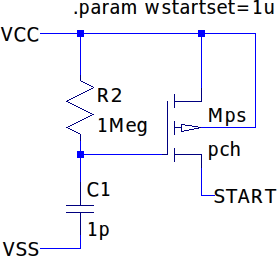
\includegraphics[scale=0.5]{spice1.png}
        \caption{Vnitřní zapojení OTA zesilovače.}
        \label{fig:spice1.png}
    \end{figure}
    
    Z analýzy .OP lze vypočítat spotřebu zapojení:
    \begin{align*}
        P&=U_{CC}\cdot (I_{p5} +I_{p3} +I_{p4} ) \\
        P&=\num{1.8}\cdot (\num{20.34e-6} +\num{21.142e-6} +\num{106.07e-6} ) \\
        P&=\qty{265.59}{\micro W} \\
    \end{align*}
